\documentclass[12pt] {article}
\usepackage[top=1.75in, bottom=1.75in, left=1.75in, right=1.75in]{geometry}
\usepackage[pdftex]{hyperref}
\usepackage{graphicx}
\usepackage{float}
\hypersetup{
	pdfauthor={Phil Monroe and Kramer Straube},
	pdftitle={Face Detection on the GPU}}
	
\begin{document}

% Title
\centerline{\Large \bf Face Detection on the GPU}

% Author
\centerline{\bf Phil Monroe and Kramer Straube}

% Date
\centerline{Mar. 15, 2012}
\bigskip

\begin{abstract}
In this paper, we implemented the beginnings of the Viola-Jones object detection method as it applies to faces. We also added a single feature classifier to detect the presence of glasses. To implement this on the GPU, we first find the integral image which is done serially because it is faster. Then, we cascade our identifiers and apply them using the integral image to minimize memory accesses. Finally, we present the list of our hypotheses for the location of the face back to the CPU. INSERT SOME JUNK ABOUT RESULTS HERE
\end{abstract}

\section{Introduction}
In this paper, we will address the application of face detection on the GPU. We used the Viola-Jones Object Detection algorithm to detect faces. We also added a glasses identifier to make an attempt at detecting whether the faces detected had glasses or not. We tested our algorithm on a subset of the Caltech Web Faces database and a subset of the Caltech 101 image database to analyze how accurate our implementation was. Finally, we discuss the pros and cons of the implementation as well as some notable aspects of our specific implementation.

\section{Viola-Jones Object Detection}
Viola-Jones object detection focuses on using simple identifiers to determine whether the object exists in the image or not. The algorithm also performs face localization if sufficiently many identifiers are used.


\subsection{Integral Image}
To speed up computation of the identifiers, the Viola-Jones algorithm pre-computes the integral image. The integral image defines each pixel as the sum of all pixels that are both above and to the left of it normalized to a maximum value in the image of one. We explored both the standard serial implementation of computing the integral image from OpenCV as well as a parallel implementation. (EXPLAIN PARALLEL IMPLEMENTATION HERE A LITTLE)


\subsection{Cascade of Identifiers}
text and figure of our identifiers
\begin{figure}[h!]
	\centering
		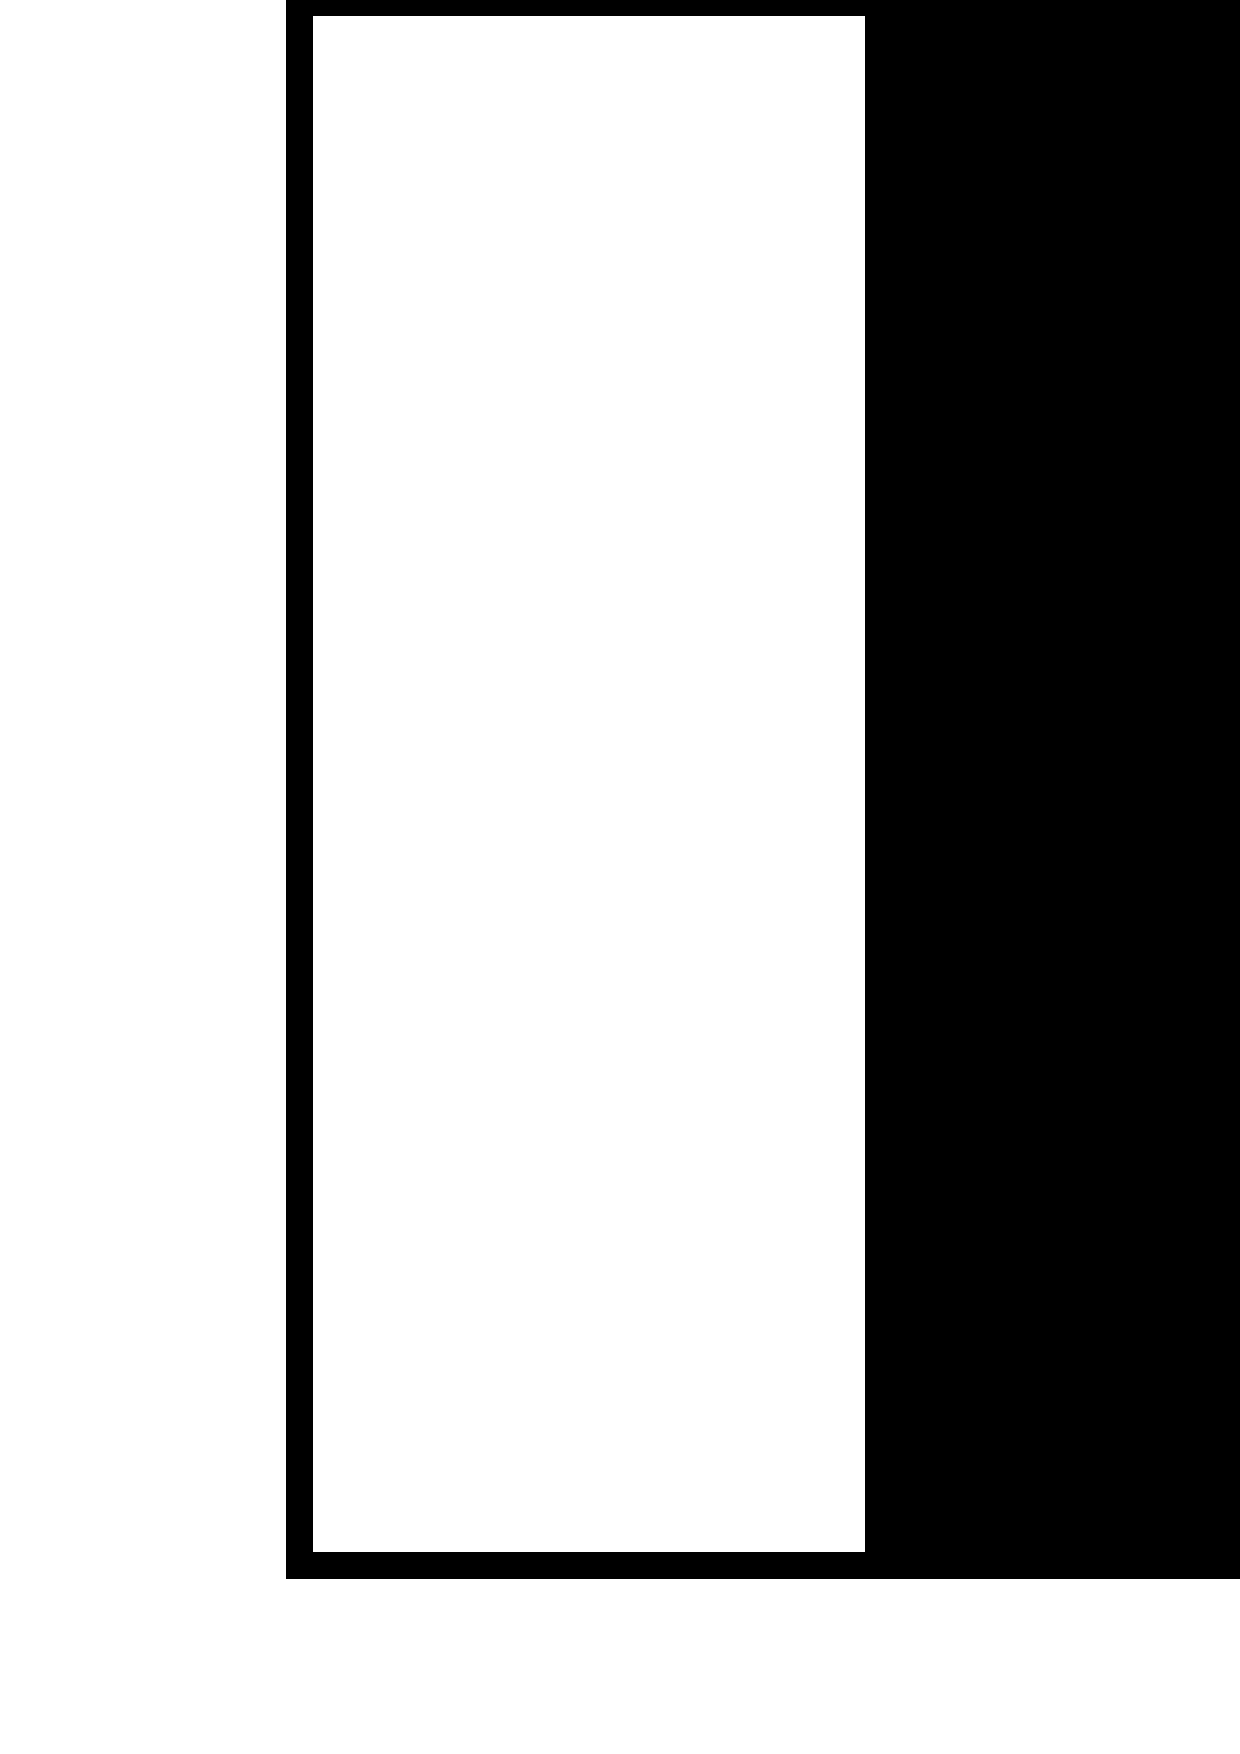
\includegraphics[width=80mm]{classifiers.pdf}
		\caption{The set of identifiers used in our implementation of Viola-Jones}
\end{figure}



\subsection{Glasses Identifier}
text and figure of our glasses identifier

\begin{figure}[h!]
	\centering
		
\includegraphics[width=40mm]{glasses_identifier.pdf}
		\caption{The glasses identifier that we implemented}
\end{figure}

\section{Results}
Stuff goes here

\section{Discussion}

\section{Conclusion}
Conclusion goes here

% References -----------------------------------------------------------------
\clearpage
\large \bf {References}
\medskip

\normalsize
\begin{itemize}
	
	\item EEC 277 Lectures 1+2 plus slides.
	
	\item David Luebke and Greg Humphrey - How GPUs Work \newline
	\url {http://bit.ly/hHt4VH}

\end{itemize}

\end{document}

